\documentclass[a4paper,12pt]{article}
\usepackage[utf8]{inputenc}
\usepackage[spanish,es-tabla]{babel}
\usepackage{color}
\usepackage{parskip}
\usepackage{graphicx}
\usepackage{multirow}
\usepackage{listings}
\usepackage{vmargin}
\usepackage{subfigure}
\graphicspath{ {imagenes/} }
\definecolor{mygreen}{rgb}{0,0.6,0}
\definecolor{lbcolor}{rgb}{0.9,0.9,0.9}
\usepackage{epstopdf}


\begin{document}
\title{Análisis y Resultados}
\author{
Christofer Fabián Chávez Carazas \\
\small{Universidad Nacional de San Agustín} \\
\small{Algoritmos Paralelos}
}

\maketitle

\section{Descripción del Problema}

Usando \textit{Pthreads} implementar tres algoritmos paralelos: Multiplicación matriz-vector, Cálculo de PI y una lista
enlazada multihilo. Para la Multiplicación matriz-vector, probar y analizar el algoritmo con diferentes tipos de tamaños.
Para el cálculo de PI, probar y analizar el algoritmo implementado con \textit{Busy-Wait} y con \textit{Mutex}.
Para la lista enlazada, probar y analizar el algoritmo implementado con los diferentes tipos de mutex. 

\section{Resultados}

\subsection{Set-Up}
\begin{itemize}
 \item Procesador: Intel(R) Core(TM) i5-4200U CPU @ 1.60GHz.
 \item Memoria: 6 Gb.
 \item L2 Cache: 3072 KB.
\end{itemize}


\subsection{Multiplicación matriz-vector}

Para implementar la multiplicación matriz-vector se repartió de manera equitativa las filas de la matriz entre los hilos.
En la Tabla \ref{tab:mv} se muestran los tiempos y la eficiencia con los diferentes tamaños de matrices y el número de
hilos. Como se puede observar la matriz cuadrada de 8000x8000 tiene los tiempos más bajos, seguido por la matriz de 8x8,000,000 y
luego la más lenta 8,000,000x8.\\
En la Figura \ref{fig:cache} se muestra los caché misses de las tres pruebas con un hilo. Con una matriz 8,000,000x8 se tienen
más \texttt{write miss} (Figura \ref{cache1}) lo que lo hace más lento. Con una matriz 8x8,000,000 y 8000x8000 se tienen
el mismo número de \textit{read miss} en el primer nivel de la cache (Figuras \ref{cache2} y \ref{cache3}), pero la diferencia
se ve en el último nivel de la cache, donde la matriz 8000x8000 tiene menos \textit{read miss}.

{%
\newcommand{\mc}[3]{\multicolumn{#1}{#2}{#3}}
\begin{table}
\begin{center}
\begin{tabular}{|c|c|l|c|l|c|l}\cline{1-3}\cline{4-5}\cline{6-7}
 & \mc{2}{c|}{8,000,000x8} & \mc{2}{c|}{8000x8000} & \mc{2}{c|}{8x8,000,000}\\\hline
Treads & Time & \mc{1}{c|}{Eff.} & Time & \mc{1}{c|}{Eff.} & Time & \mc{1}{c|}{Eff.}\\\hline
1 & 0.851185 & \mc{1}{c|}{1} & 0.298461 & \mc{1}{c|}{1} & 0.401316 & \mc{1}{c|}{1}\\\hline
2 & 0.596006 & \mc{1}{c|}{0.7140741872} & 0.176037 & \mc{1}{c|}{0.8477223538} & 0.326044 & \mc{1}{c|}{0.6154322729}\\\hline
4 & 0.534235 & \mc{1}{c|}{0.3983195597} & 0.16622 & \mc{1}{c|}{0.4488945374} & 0.285785 & \mc{1}{c|}{0.3510646115}\\\hline
\end{tabular}
\end{center}
\caption{Run-Times y eficiencia de la Multiplicación Matriz-Vector}
\label{tab:mv}
\end{table}
}%

\begin{figure}
  \centering
  \subfigure[Caché misses con matriz 8,000,000x8]
    {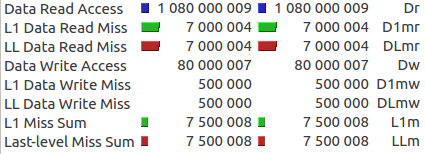
\includegraphics[scale=0.5]{cache1.png}
    \label{cache1}
   }
  \subfigure[Caché misses con matriz 8000x8000]{
    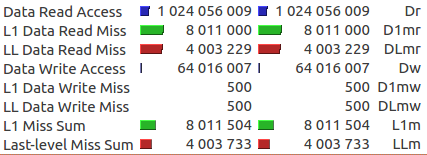
\includegraphics[scale=0.5]{cache2.png}
    \label{cache2}
   }
   \subfigure[Caché misses con matriz 8x8,000,000]{
    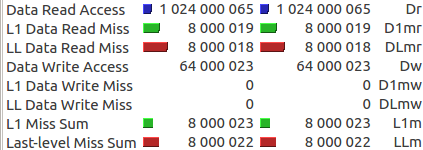
\includegraphics[scale=0.5]{cache3.png}
    \label{cache2}
   }
  \caption{Resultados del Valgrind para la Multiplicación Matrix-Vector con un hilo}
  \label{fig:cache}
\end{figure}

\subsection{Cálculo de PI}

Se probó el programa con dos implementaciones, uno con espera activa y otro utilizando mutex, los dos colocados donde el
hilo actualiza la variable global. El experimento se ejecutó con un $n = 10^{8}$. Los resultados se muestran en la Tabla 
\ref{tab:pi}. Como se puede ver, con pocos hilos no hay mucha diferencia en el tiempo, pero cuando se va incrementando el
número de hilos, la espera activa demora mucho más. Esto se debe a que el mutex, cuando se desbloquea, deja que cualquier
hilo que este esperando entre, pero la espera activa sólo deja entrar al hilo con el id siguiente.

\begin{table}
\begin{center}
\begin{tabular}{|c|c|c|}\hline
Threads & Busy-Wait & Mutex\\\hline
1 & 1.417573 & 1.410313\\\hline
2 & 0.845606 & 0.840515\\\hline
4 & 0.758986 & 0.75207\\\hline
8 & 0.845326 & 0.724456\\\hline
16 & 0.889439 & 0.703118\\\hline
32 & 1.031882 & 0.728032\\\hline
64 & 1.678438 & 0.715238\\\hline
\end{tabular}
\end{center}
\caption{Run-Times (en segundos) del cálculo de PI}
\label{tab:pi}
\end{table}

\subsection{Lista enlazada}

Se probó el programa con tres implementaciones: un mutex para toda lista, un mutex para cada nodo de la lista, y
un \textit{read-write lock}. Los experimentos se hicieron con una lista enlazada con 1000 elemento iniciales generados
aleatoriamente. Para cada ejecución se computó un total de 100,000 operaciones de Member, Insert y Delete, variando el
porcentaje de operaciones a ejecutar. Todos los hilos se reparten equitativamente las operaciones; todos los hilos hacen las
tres operaciones en porciones iguales. \\
En las Tablas \ref{tab:list1} y \ref{tab:list2} se muestras los tiempos con las diferentes implementaciones, el número de 
hilos y los diferentes porcentajes para cada operación. En todos los casos poner un mutex por nodo demora más y es más costoso,
por lo que no es muy recomendable usarlo. Cuando hay un número considerable de operaciones de lectura (Tabla \ref{tab:list1}),
la implementación con read-write lock es un poco más rapida que la implementación con un sólo mutex para toda la lista, casi
no habiendo mucha diferencia. Pero cuando el número de operaciones de lectura es muy pequeño (Tabla \ref{tab:list2}), sí se nota 
la diferencia, siendo la implementación con read-write locks mucho más rápida.



{%
\newcommand{\mc}[3]{\multicolumn{#1}{#2}{#3}}
\begin{table}
\begin{center}
\begin{tabular}{|c|c|lll}\cline{1-5}
 & \mc{4}{c|}{\textbf{Number of Threads}}\\\hline
\textbf{Implementation} & 1 & \mc{1}{c|}{2} & \mc{1}{c|}{4} & \mc{1}{c|}{8}\\\hline
Read-Write Locks & 0.606194 & \mc{1}{c|}{0.917242} & \mc{1}{c|}{0.974216} & \mc{1}{c|}{1.031685}\\\hline
One Mutex for Entire List & 0.641805 & \mc{1}{c|}{1.151787} & \mc{1}{c|}{1.094305} & \mc{1}{c|}{1.197174}\\\hline
One Mutex per Node & 2.004661 & \mc{1}{c|}{5.108905} & \mc{1}{c|}{6.368233} & \mc{1}{c|}{4.163973}\\\hline
\end{tabular}
\end{center}
\caption{Tiempos de la lista enlazada con 80\% Member, 10\% Insert, 10\% Delete}
\label{tab:list1}
\end{table}
}%

{%
\newcommand{\mc}[3]{\multicolumn{#1}{#2}{#3}}
\begin{table}
\begin{center}
\begin{tabular}{|c|c|ccc}\cline{1-5}
 & \mc{4}{c|}{\textbf{Number of Threads}}\\\hline
\textbf{Implementation} & 1 & \mc{1}{c|}{2} & \mc{1}{c|}{4} & \mc{1}{c|}{8}\\\hline
Read-Write Locks & 0.195334 & \mc{1}{c|}{0.257124} & \mc{1}{c|}{0.302961} & \mc{1}{c|}{0.296626}\\\hline
One Mutex for Entire List & 0.192306 & \mc{1}{c|}{0.539524} & \mc{1}{c|}{0.530687} & \mc{1}{c|}{0.549751}\\\hline
One Mutex per Node & 1.67227 & \mc{1}{c|}{2.546439} & \mc{1}{c|}{3.03843} & \mc{1}{c|}{3.428606}\\\hline
\end{tabular}
\end{center}
\caption{Tiempos de la lista enlazada con 99.9\% Member, 0.05\% Insert, 0.05\% Delete}
\label{tab:list2}
\end{table}
}%




\end{document}
